\documentclass[12pt]{article}
\usepackage{tikz}
\usepackage{pgfplots}
\pgfplotsset{compat=1.13}

\usepackage{extsizes}
\usepackage{caption}
\usepackage{multirow}
\usepackage{wrapfig}

\renewcommand{\epsilon}{\ensuremath{\varepsilon}}
\renewcommand{\phi}{\ensuremath{\varphi}}
\renewcommand{\kappa}{\ensuremath{\varkappa}}
\renewcommand{\le}{\ensuremath{\leqslant}}
\renewcommand{\leq}{\ensuremath{\leqslant}}
\renewcommand{\ge}{\ensuremath{\geqslant}}
\renewcommand{\geq}{\ensuremath{\geqslant}}
\renewcommand{\emptyset}{\varnothing}

\newcommand{\lw}{\linewidth}
\usepackage{geometry} % Простой способ задавать поля
\geometry{top=30mm}
\geometry{bottom=30mm}
\geometry{left=25mm}
\geometry{right=20mm}

\usepackage[T2A]{fontenc}			% кодировка
\usepackage[utf8]{inputenc}	
\usepackage[english,russian]{babel}   %% загружает пакет многоязыковой вёрстки
\usepackage{indentfirst}
\usepackage{subfigure}
\usepackage{amsmath,amsfonts,amssymb,amsthm,mathtools} 
\usepackage{graphicx}

\usepackage{pdfpages}

\title{Задача к собеседованию на ИППИ}
\author{Самохин В.~Ю.}
\begin{document}
	\maketitle
	\paragraph{Задача. }
	Задача классификации заключается в том, что по выборке данных $$\{(\mathbf{x}_i, y_i = y(\mathbf{x}_i))\}_{i=1}^{n}, \; \mathbf{x}_i \in \mathbb{R}^d,\ y_i \in \{-1,1\}$$
	необходимо построить модель зависимости $\hat{y}(\mathbf{x})$ такую, что $\hat{y}(\mathbf{x}) \in \{-1,1\}$ и для большинства значений $\mathbf{x}$ прогноз метки класса $\hat{y}(\mathbf{x})$ совпадает с настоящей меткой класса $y(\mathbf{x})$.
	
	Рассматривает модель линейной разделяющей гиперплоскости $$\hat{y}(\mathbf{x}) = sign(\mathbf{x}_i^T\mathbf{w} + w_0 > 0)$$
	
	Для оценки вектора параметров $\mathbf{w}, w_0$ максимизируется отступ разделяющей гиперплоскости от объектов обучающей выборки:
	
	$$\underset{\mathbf{w}, w_0, ||\mathbf{w}|| = 1}{\max}M,$$
	$$s.t. \ y_i(\mathbf{x}_i^T\mathbf{w} + w_0) \geq M, \; i = \overline{1,n}.$$
	
	Нужно описать, как решать такую задачу оптимизации и какими свойствами обладает ее решение.
	
	\paragraph{Решение}
	
	Нужно понимать, что выражение $y_i(\mathbf{x}_i^T\mathbf{w} + w_0)$ является отступом, и когда выражение является отрицательным, это означает, что алгоритм допустил ошибку. При этом можно сказать, что чем больше отступ, тем больше алгоритм уверен в своем прогнозе.
	Наша задача заключается в том, чтобы найти такую гиперплоскость, разделяющую два класса, чтобы расстояния до нее от любой точки выборки было максимальным.
	
	Условия, наложенные на $\mathbf{w}, w_0$, можно заменить следующим образом. Вместо использования ограничений, поделим обе части неравенства на модуль вектора весов.
	Получим эквивалентное неравенство:
	$$\dfrac{1}{||\mathbf{w}||} y_i(\mathbf{x}_i^T\mathbf{w} + w_0) \geq M,$$
	или, взяв $||\mathbf{w}|| = \frac{1}{M}$,
		$$\underset{\mathbf{w}, w_0}{\min} ||\mathbf{w}||^2,$$
	$$s.t. \ y_i(\mathbf{x}_i^T\mathbf{w} + w_0) \geq 1, \; i = \overline{1,n}.$$
	
	Теперь нам необходимо решить задачу минимизации при заданном условии.
	
	Заметим, что оптимизируемая функция выпуклая, поскольку гессиан является положительно определенной формой.
	Поскольку накладываемое ограничение в задаче условного экстремума - неравенство, то уместно записать функцию Лагранжа и условие Каруша-Куна-Таккера\footnote{Использовалась соответствующая статья на Википедии}, которым должно удовлетворять решение этой функции.
	
	$$L = \dfrac{1}{2}||\mathbf{w}||^2 - \sum_{i=1}^{N}\lambda_i(y_i(\mathbf{x}_i^T\mathbf{w} + w_0) - 1)$$
	
	Условия:
	\begin{itemize}
		\item стационарности: $\underset{\mathbf{x}}{\max}\ L = L(\hat{\mathbf{x}})$
		\item дополняющей нежесткости: $\lambda_i(y_i(\mathbf{x}_i^T\mathbf{w} + w_0) - 1) = 0, \; i = \overline{1,N}$
		\item неотрицательности: $\lambda_i \geq 0,  \; i = \overline{1,N}$
	\end{itemize}

	Из условия стационарности мы должны приравнять производные к нулю по $\mathbf{w}$ и $w_0$. 
	\begin{align}
	\label{eq::derivatives}
\mathbf{w} = \sum_{i=1}^{N}\lambda_i y_i \mathbf{x}_i
\\
	 0 = \sum_{i=1}^{N}\lambda_i y_i
	\end{align}	
	Подставив эти значения в функцию Лагранжа, получим
	$$L = \sum_{i=1}^{N}\lambda_i - \dfrac{1}{2}\sum_{i=1}^N\sum_{k=1}^N\lambda_i\lambda_ky_iy_k\mathbf{x}_i^T\mathbf{x}
_k,$$ и теперь нужно минимизировать $-L$ при $\lambda_i \geq 0$.

Теперь вернемся к рассмотрению условий. Из второго условия следует, что либо $(y_i(\mathbf{x}_i^T\mathbf{w} + w_0) = 1$ при $\lambda_i > 0$, то есть $\mathbf{x}_i$ лежит на \textit{границе} разделяющей области, либо $(y_i(\mathbf{x}_i^T\mathbf{w} + w_0) > 1$ при $\lambda_i = 0$, и тогда объект на границе не лежит. 

Что нам это дает? Вернемся к уравнениям \eqref{eq::derivatives}. Видим, что вектор $\mathbf{w}$ есть линейной комбинацией  так называемых \textit{опорных объектов}, для которых выполнено условие $\lambda_i \neq 0$.

\begin{center}
	

	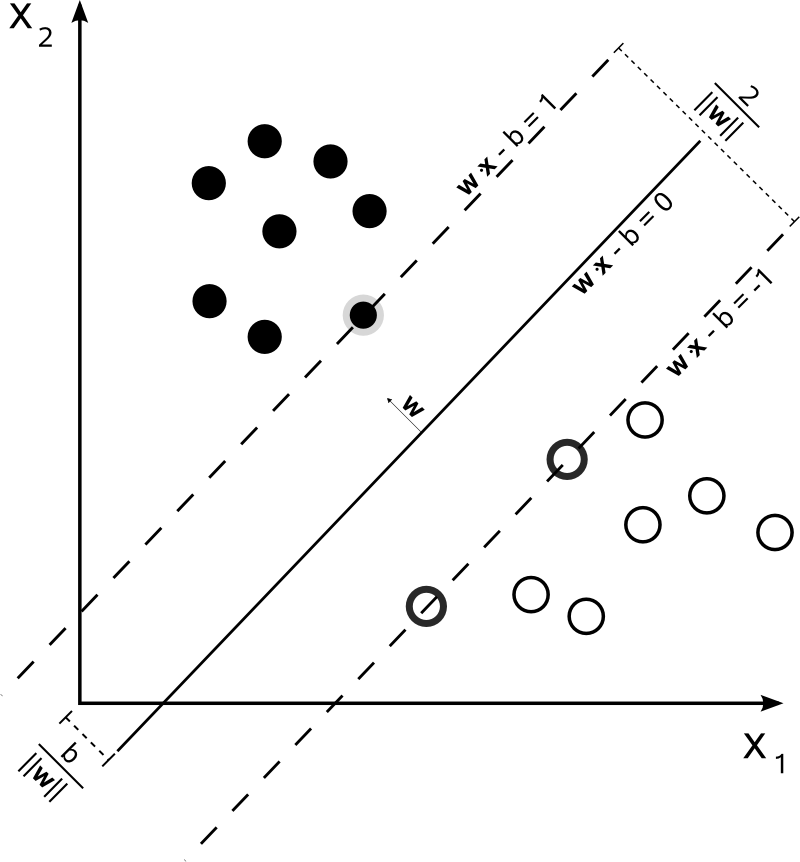
\includegraphics[scale=0.5]{hyperplane}
	\captionof{figure}{Разделяющая прямая в двухмерном случае. На границе разделяющей области - опорные векторы}

\end{center}
Чтобы найти $w_0$, нужно решить условие дополнительной нежесткости для одного из опорных объектов.


\subparagraph{Неразделимые классы.}
На практике объекты двух классов не всегда можно разделить гиперплоскостью из-за зашумленности данных. Тогда нужно разрешить классификатору допускать ошибки, при этом можно ввести цену такой ошибок.

При этом мы хотим заплатить как можно меньшую цену.

По аналогии с идеальным случаем получим следующую задачу с переменными $\mathbf{w}, w_0, \mathbf{\xi}$, а также ценой ошибки $C$:
\begin{align*}&
\underset{\mathbf{w}, w_0}{\min} \dfrac{1}{2}||\mathbf{w}||^2 + C\sum_{i=1}^N \xi_i,
\\&s.t. \xi_i \geq 0,\; y_i(\mathbf{x}_i^T\mathbf{w} + w_0) \geq 1 - \xi_i, \; i = \overline{1,n}.
\end{align*}

Теперь у нас лобавилось условие на $\xi_i$. Функция Лагранжа для данной задачи примет вид 
$$L = \dfrac{1}{2}||\mathbf{w}||^2 + C\sum_{i=1}^N\xi_i - \sum_{i=1}^N\lambda_i(y_i(\mathbf{x}_i\mathbf{w} + w_0) - (1-\xi_i)) - \sum_{i=1}^{N}\mu_i\xi_i$$

Приравняв к нулю производные, получим
\begin{align}
\label{eq::new_derivative}
\mathbf{w} &= \sum_{i=1}^{N}\lambda_i y_i \mathbf{x}_i
\\
0 &= \sum_{i=1}^{N}\lambda_i y_i
\\
\lambda_i &= C - \mu_i
\end{align}

Сделав необходимые замены, получим функцию Лагранжа в следующем виде
$$L = \sum_{i=1}^{N}\lambda_i - \dfrac{1}{2}\sum_{i=1}^N\sum_{k=1}^N\lambda_i\lambda_ky_iy_k\mathbf{x}_i^T\mathbf{x}
_k,$$
Добавим к этому условия Каруша-Куна-Таккера, которые должны выполняться для любого решения задачи

\begin{itemize}

\item дополняющей нежесткости:
\begin{itemize}
	\item 
 $\lambda_i(y_i(\mathbf{x}_i^T\mathbf{w} + w_0) - (1-\xi_i)) = 0, \; i = \overline{1,N}$
 \item $\mu_i\xi_i = 0$
\end{itemize}
\item неотрицательности: $\lambda_i \geq 0,  \; i = \overline{1,N}$,


\end{itemize}
мы снова получим результат, при котором $\mathbf{w}$ есть линейная комбинация \textit{опорных векторов}.

\paragraph{Случай с заданными весами}

Допустим, что у объектов есть положительные веса, с помощью которых можно задать, для каких объектов из обучающей выборки важнее всего получить точную классификацию.

В такой постановке задачи меняется обучающая выборка: вместе с описанием объектов и целовой переменной появляется дополнительный параметр весов точек. 

Однако основной принцип остается тем же: мы продолжаем разрешать классификатору допускать ошибки, но теперь их стоимость различается для всех объектов выборки. 

Запишем задачу:

\begin{align*}&
\underset{\mathbf{w}, w_0}{\min} \dfrac{1}{2}||\mathbf{w}||^2 + C\sum_{i=1}^N W_i\xi_i,
\\&s.t. \xi_i \geq 0,\; y_i(\mathbf{x}_i^T\mathbf{w} + w_0) \geq 1 - \xi_i, \; i = \overline{1,n}.
\end{align*}
За $W_i$ обозначен вес  $i$-го объекта.

Функция Лагранжа для данной задачи примет вид 
$$L = \dfrac{1}{2}||\mathbf{w}||^2 + C\sum_{i=1}^NW_i\xi_i - \sum_{i=1}^N\lambda_i(y_i(\mathbf{x}_i\mathbf{w} + w_0) - (1-\xi_i)) - \sum_{i=1}^{N}\mu_i\xi_i$$

Приравняв к нулю производные, получим
\begin{align}
\mathbf{w} &= \sum_{i=1}^{N}\lambda_i y_i \mathbf{x}_i
\\
0 &= \sum_{i=1}^{N}\lambda_i y_i
\\
\lambda_i &= CW_i - \mu_i
\end{align}

КТ-условия не изменятся, напомню их

\begin{itemize}
	
	\item дополняющей нежесткости:
	\begin{itemize}
		\item 
		$\lambda_i(y_i(\mathbf{x}_i^T\mathbf{w} + w_0) - (1-\xi_i)) = 0, \; i = \overline{1,N}$
		\item $\mu_i\xi_i = 0$
	\end{itemize}
	\item неотрицательности: $\lambda_i \geq 0,  \; i = \overline{1,N}$,
	
	
\end{itemize}


Получили, что единственная разница по сравнению с предыдущим случаем - другое ограничение на $\lambda_i$, верхняя граница стала динамической, то есть она различна жля каждой точки.

Интересно заметить, что существенным является значение константы $C$.  При $C \to 0$ или $C \to +\infty$ окажется, что $CW_i = C$, и значит влияние весов учтено не будет. 

\end{document}